\chapter{接通在线规划与完整导航}
\begin{notebox}
\textbf{目标}\quad 将定位、地图、局部规划和跟踪连成闭环；理解未来参考接续、坐标冻结与导航误差的计算。\\
\textbf{先修}\quad 第 08--18 章。先运行参考交接例子，再启动完整导航，最后比较不同机器人模型。
\end{notebox}
\section{运动带来新观测，新观测改变下一次计划}
前几章分别建立了传感器、估计器、地图、轨迹和控制器。
导航把它们连接起来：机器人向前走，看见原来被遮挡的区域；新地图又改变接下来可走的路线。
规划因此需要反复更新，而控制器在计算新计划期间仍要持续跟踪已有参考。

\begin{center}\begin{minipage}{\linewidth}\makeatletter\def\@captype{figure}\makeatother
\centering
\begin{tikzpicture}[>=Stealth,node distance=.55cm,
 b/.style={draw=tealblue,fill=pale,rounded corners,minimum width=2.05cm,minimum height=.85cm,align=center,font=\small}]
\node[b] (s) {激光与 IMU};\node[b,right=of s] (m) {定位与地图};
\node[b,right=of m] (p) {局部规划};\node[b,right=of p] (c) {跟踪控制};\node[b,right=of c] (r) {机器人};
\draw[->] (s)--(m);\draw[->] (m)--(p);\draw[->] (p)--(c);\draw[->] (c)--(r);
\draw[->] (r.south)--++(0,-.8)-| (s.south);
\node[fill=white,font=\small] at(5.2,-.8) {运动改变下一帧观测};
\node[above=.5cm of p,font=\small] (g) {地图中的目标};\draw[->] (g)--(p);
\end{tikzpicture}
\caption{导航的闭环关系。定位产生的当前状态同时供规划和控制使用；地图描述机器人已经观测到的空间。}
\end{minipage}\end{center}
每个模块使用不同的时间尺度：IMU 与动力学更新较快，激光和地图较慢，优化还需要计算时间。
本章先解决参考如何在未来时刻平滑交接，再解释规划时使用哪一份地图，以及控制器如何接收这个计划。

\section{新曲线从未来交接状态出发}
\begin{lstlisting}[language=bash,numbers=none]
ros2 run motion2d reference_handover_demo tmp/ch19_handover
/usr/bin/python3 scripts/plot_ch19_handover.py
\end{lstlisting}
设现在的绝对仿真时间为 $t_0$，预留 $\Delta>0$ 的计算和传输时间，计划在 $t_s=t_0+\Delta$ 交接。
旧曲线的绝对起点为 $t_b$，因此它在交接处的局部时间是 $\tau_s=t_s-t_b$。
新曲线的局部时间则从零开始，首边界应设为
\begin{equation}
 p_n(0)=p_o(\tau_s),\qquad v_n(0)=v_o(\tau_s),\qquad a_n(0)=a_o(\tau_s).\label{eq:handover}
\end{equation}
整体参考为 $p(t)=p_o(t-t_b)$（$t<t_s$）和 $p(t)=p_n(t-t_s)$（$t\geq t_s$）。
从左右分别取极限，式\eqref{eq:handover}使位置及其一、二阶导数都相等，这就是 $C^2$ 接续。
由 $F=ma+c_vv$，模型匹配时的平移前馈力也连续。
jerk 是加速度的导数；当前边界没有匹配它，因此力的变化率可能在交接处改变。

\subsection{在旧曲线上手算首边界}
示例旧曲线从 $(0,0)$ 静止走到 $(2,0)$，时长 4 s。
用第 14 章的 $h(s)=10s^3-15s^4+6s^5$，有 $p_x=2h(t/4)$。
在绝对起点为零、$t_s=1.5$ s 时，$s=3/8$，逐项求导得到
\[
 p_x=2h(3/8)=0.550415\text{ m},\quad
 v_x=\tfrac24h'(3/8)=0.823975\text{ m/s},\quad
 a_x=\tfrac2{16}h''(3/8)=0.439453\text{ m/s}^2.
\]
新曲线从这组边界出发，用 4 s 转向 $(3,1)$ 并停下。
如果只匹配位置而把新速度设成零，参考速度会跳变约 0.824 m/s；在 0.02 s 的控制间隔上，
对应约 41.2 m/s$^2$ 的速度变化要求。保留旧参考的导数能避免这种人为突变。
\begin{center}\begin{minipage}{\linewidth}\makeatletter\def\@captype{figure}\makeatother
\centering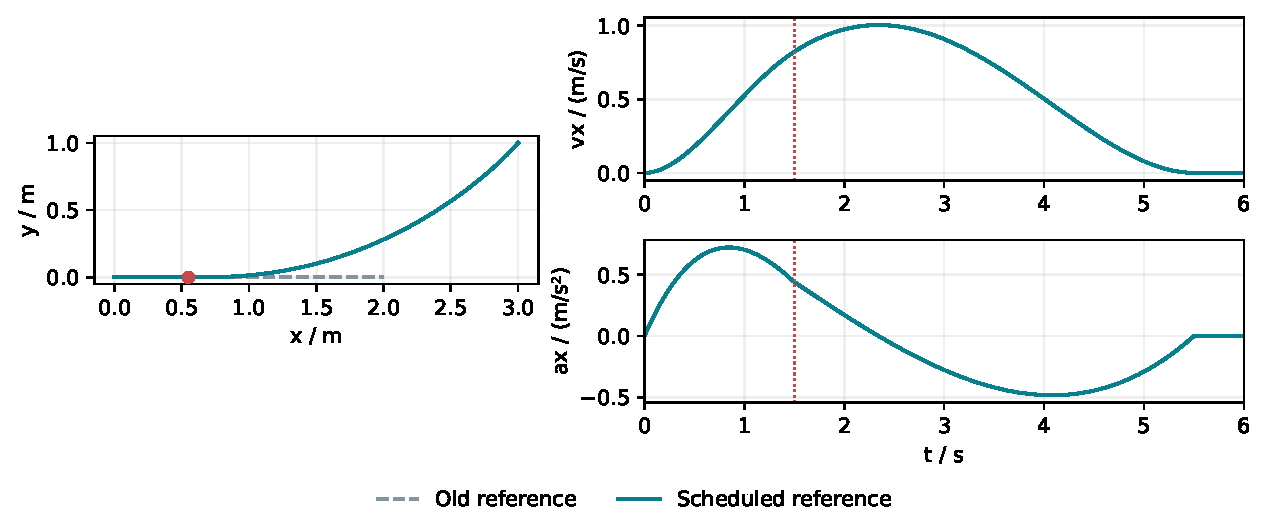
\includegraphics[width=\linewidth]{figures/ch19_handover.pdf}
\caption{在 1.5 s 交接。旧曲线原本沿 x 轴到达 (2,0)，新曲线转向 (3,1)；
红点和竖虚线标记交接时刻。速度与加速度保持连续，jerk 不要求连续。}
\end{minipage}\end{center}
规划计算期间继续执行旧曲线，反馈处理实际状态相对旧参考的偏差。
如果偏差已使现有走廊余量不足，则先制动、重新静止定位，再建立下一条参考。
这一操作与平滑接续分别对应两种控制状态，应在状态记录和误差曲线上标出。

\section{查询未来与推进当前是两件操作}
MPC 在时刻 $t_0$ 就会查询 $t_0+h,\ldots,t_0+Nh$，其中可能有时刻已经越过 $t_s$。
调度器需要按查询时间返回正确曲线，同时保留真正的当前活动曲线。
\code{ReferenceSchedule} 保存 \code{active} 与至多一条 \code{pending}，其行为可按时间表理解：
\begin{center}\small
\begin{tabular}{lll}\toprule
实际观测时刻 & 查询时刻 & 应返回的参考\\\midrule
1.2 s & 1.3 s & 旧曲线\\
1.2 s & 1.6 s & 未来候选，但保留旧活动曲线\\
1.2 s & 1.2 s & 仍为旧曲线\\
1.5 s & 1.6 s & 已交接的新活动曲线\\\bottomrule
\end{tabular}
\end{center}
\code{sample} 是只读查询，\code{advance} 由实际推进的观测时刻调用，达到 $t_s$ 才把候选变成活动曲线。
接收新曲线时，先用同一绝对起点查询旧参考，再检查首边界：
\par\noindent\begin{minipage}{\linewidth}
\lstinputlisting[language=C++,linerange={reference_handover_begin-reference_handover_end},includerangemarker=false]{../ros2_ws/src/motion2d/src/trajectory/reference_schedule.cpp}
\end{minipage}\par
三个范数分别比较位置、速度和加速度，最后还匹配固定 yaw。
$10^{-7}$ 用于数值计算后的同一边界比较；每项保持自己的 SI 单位。
终点 v/a 必须为零，这样到达以后可接上恒定位置保持。
起点已经过去、第二条候选仍待交接或边界不匹配时，保留原有效计划并返回原因；
显式 \code{reset} 则清空两条参考，把静止锚点设为新的位姿。

\section{规划时冻结 map 与 odom 的变换}
回环校正改变地图与局部里程计之间的对齐。设本次规划采用
\[
 p_m=Rp_o+b,
\]
其中 $R,b$ 在本次求解和参考转换中保持固定。由 $R^TR=I$，反解并对时间求导：
\begin{equation}
 p_o=R^T(p_m-b),\qquad v_o=R^Tv_m,\qquad a_o=R^Ta_m.\label{eq:navframe}
\end{equation}
位置含平移，导数中的常量平移消失。
将 $p_m(t)=\sum_{k=0}^5c_{m,k}t^k$ 代入，逐次幂收集，得到
\[
 c_{o,0}=R^T(c_{m,0}-b),\qquad c_{o,k}=R^Tc_{m,k}\quad(k\geq1).
\]
走廊顶点也使用同一变换，再重新构造半空间；固定 yaw 减去 $R$ 对应的旋转角。

例如 $R$ 表示 $90^\circ$ 旋转、$b=(1,2)$，地图位置 $(1,3)$、速度 $(0,0.5)$
转换为 odom 位置 $(1,0)$、速度 $(0.5,0)$。
若下一次地图平移校正为 $(1.1,2)$，把旧地图系数直接重新转换会让其 odom 位置跳到 $(1,0.1)$。
因此已发送的 odom 系数保持固定；新的变换用于下一次规划，并从旧 odom 参考的未来边界接续。

\code{transformReference} 对曲线与各区域统一转换。
新地图到达后，还要把剩余 odom 区域按当前对齐放回 map，检查它们是否仍在新的自由配置空间中。
这样既保留控制参考的连续性，也及时响应新发现的障碍。

\section{在已观测空间中选一个可达的局部目标}
\begin{lstlisting}[language=bash,numbers=none]
ros2 run motion2d replanner_demo tmp/ch19_replanner
/usr/bin/python3 scripts/plot_ch19_replanner.py
\end{lstlisting}
一次规划读取同一时刻的地图快照：原始占据栅格、由它膨胀的配置空间栅格、同源未膨胀 ESDF。
原始栅格回答哪里未知、哪里有障碍；膨胀栅格回答圆心可经过哪里；ESDF 给出优化所用的距离与梯度。
这些数据来自同一份地图，才能让路径搜索和曲线检查使用一致的几何。

从未来交接点所在自由格做八邻接可达搜索，斜向连接按第 11 章禁止切角。
如果全局目标已可达，直接用 A* 搜索它；否则在可达自由格中选择邻近未知区的\textbf{前沿候选}。
因为未知区周围已经膨胀，候选不一定紧挨原始未知格。代码检查的窗口半径为
\[
 n_w=\left\lceil\frac{r_{\rm clearance}}{d}\right\rceil+2,
\]
$d$ 为分辨率。除以 $d$ 把米换成格数，向上取整覆盖膨胀距离，额外两格容纳格子边界与搜索邻域。
例如 $r_{\rm clearance}=0.15$ m、$d=0.1$ m，得到四格窗口。

对候选中心 $q$ 比较 $\|q-g\|^2$，选离全局目标 $g$ 最近者。
平方距离与距离的大小顺序相同，省去了逐候选开方。
还要求 $\|p_s-g\|-\|q-g\|\geq0.1$ m，避免在几乎不前进的候选间反复切换。
在需要先远离目标才能绕出的凹形环境中，这一规则可能停滞；可进一步加入访问历史或信息增益来改进探索。

\begin{center}\small
\begin{tabular}{lp{8.5cm}}\toprule
局部搜索状态 & 可以据此检查什么\\\midrule
no\_reachable\_frontier & 已可达自由区内没有邻近未知区的候选；查看遮挡和地图边界\\
no\_progress\_frontier & 候选离目标的改善小于阈值；查看是否需要先绕远\\
goal\_occupied / goal\_outside\_map & 目标在当前占据格或地图范围之外；重新选目标\\\bottomrule
\end{tabular}
\end{center}
搜索得到折线后，沿长度截取局部前缀，默认最多 2 m。
若已累计长度 $L$，下一段向量为 $d_p$，而剩余长度 $\ell_{\max}-L<\|d_p\|$，截断点是
\[
 q_{\rm cut}=q_{\rm last}+\frac{\ell_{\max}-L}{\|d_p\|}d_p.
\]
比例位于 $[0,1]$，所以新点仍在已经检查过的自由线段上。
例如剩 0.5 m、下一段为 $(0.6,0.8)$ m，其长度为 1 m，只走 $(0.3,0.4)$ m。
\begin{center}\begin{minipage}{\linewidth}\makeatletter\def\@captype{figure}\makeatother
\centering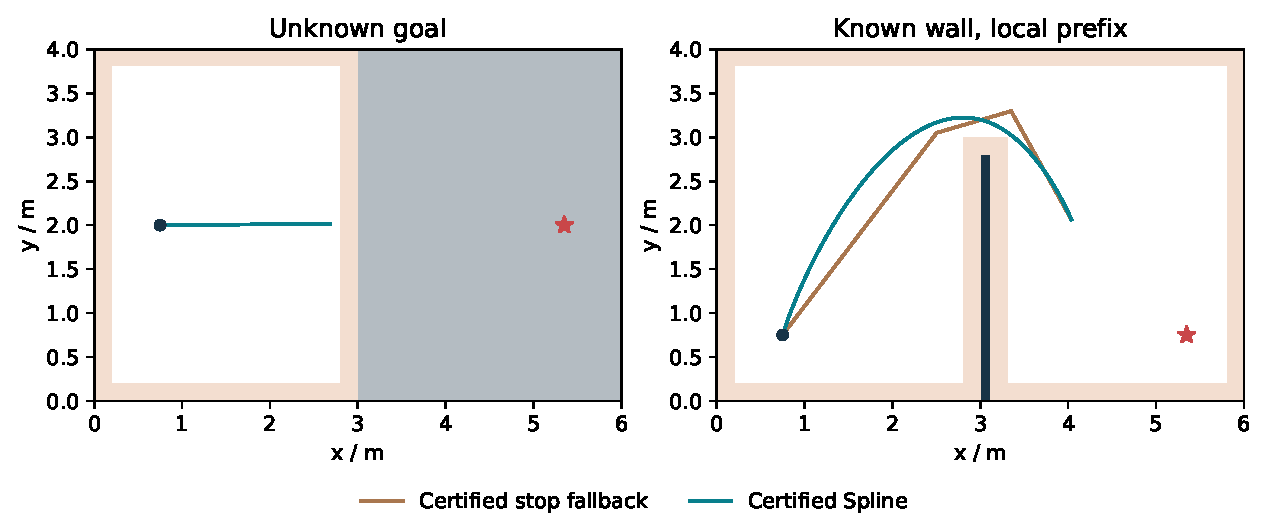
\includegraphics[width=\linewidth]{figures/ch19_replanner.pdf}
\caption{两张用于学习局部目标选择的占据网格。灰色未知、深蓝占据、浅橙为配置空间阻塞；
星号是全局目标，曲线只到达当前局部终点。左图不穿越未知区，右图采用最多 5 m 的路线前缀绕墙。}
\end{minipage}\end{center}
图中网格为 $60\times40$、分辨率 0.1 m，机器人半径 0.1 m、额外余量 0.05 m。
左侧只有 $x<3$ m 已观测，局部目标逐渐靠近未知边缘；右侧全图已知，演示最多 5 m 的绕墙路线前缀。
新的扫描扩展自由空间后，再用新快照选择下一段目标。

\section{从未来边界生成并检查局部曲线}
对局部路线构建凸走廊，起点使用式\eqref{eq:handover}的未来 p/v/a，终点设为静止。
Spline 优化使用第 15、16 章的能量、ESDF、走廊及导数代价。
核心演示默认控制点走廊权重 50000、额外内缩 0.04 m，软速度/加速度目标 0.45/0.5，
最终连续上界要求速度 0.7 m/s、加速度 0.8 m/s$^2$。
软目标帮助求解靠近可行区域，Bézier 连续界再逐段检查最终曲线。

优化结果未通过时，备用方案在各路点停下，\textbf{首段仍保留旧参考的 p/v/a}。
依次尝试基准时长及其 1.5、2、3 倍，并对每条候选作同样的连续检查。
\par\noindent\begin{minipage}{\linewidth}
\lstinputlisting[language=C++,linerange={replanner_fallback_begin-replanner_fallback_end},includerangemarker=false]{../ros2_ws/src/motion2d/src/planning/replanner.cpp}
\end{minipage}\par
\code{left=start} 保留移动起点；\code{right} 的导数默认零。
只有第一段之后，左边界才变成刚构造的静止右边界。
\code{certifyBezier} 检查同一组区域和导数限制，成功时才返回候选。

\subsection{为什么延长时长有时会把曲线推出走廊}
静止到静止时，同一形状可以通过延长时间降低导数。
但首速度 $v_0$ 已经固定时，曲线形状也随时长变化。用单轴起点位置零、首加速度零、终点位置 $D$ 且静止的五次段说明。
由第 14 章端点公式，令 $s=t/T$，可整理为
\[
 p(t)=D h(s)+v_0T b(s),\quad
 b(s)=s-6s^3+8s^4-3s^5.
\]
$h$ 提供静止到静止的位移；$b(0)=b(1)=0,b'(0)=1,b'(1)=0,b''(0)=b''(1)=0$，
因此第二项恰好补上首速度 $v_0$，其余边界保持不变。
在中点 $h(1/2)=1/2,b(1/2)=5/32$，所以
\[
 p(T/2)=D/2+5v_0T/32.
\]
取 $D=1$ m、$v_0=0.5$ m/s，$T=2$ s 时中点为 0.65625 m，$T=8$ s 时却到 1.125 m。
较长时间让初始速度带来更大的前冲。备用时长每改一次，都要重新检查空间与动力学界。

局部例子的总时长如下，优化目标包含平滑性与软约束，因此时间会随整个目标的权衡变化。
\begin{center}\small
\begin{tabular}{lrr}\toprule
场景 & 逐段停车/s & Spline/s\\\midrule
未知目标的局部前缀 & 7.258 & 11.424\\
绕墙的 5 m 前缀 & 19.466 & 12.994\\\bottomrule
\end{tabular}\end{center}
这组演示关闭优化墙钟预算以便观察解的差别；在线节点另设计算预算。
返回状态区分 \code{optimized} 与 \code{fallback_stop_segments}，并保存优化器原始状态。
所有候选都未通过时，上层进入制动与静止重试。

\section{把曲线与走廊一起交给控制器}
一条执行参考需要同时说明曲线、绝对起点、对应区域和地图快照时刻。
\code{NavigationReference} 将这些内容放在同一消息中，让控制器收到的是一套配对数据。
否则两条独立话题的到达次序可能把新曲线与旧走廊配在一起。
区域顶点采用 float64，与曲线计算保持相同精度。

接收器先检查坐标、分段与区域数量，再检查曲线在区域中的连续界，以及未来交接的 p/v/a/yaw。
接收成功后发布携带绝对起点纳秒的确认。
规划端收到匹配的确认，才将候选放进自己的参考调度，从而与控制端保持一致。

\begin{center}\begin{minipage}{\linewidth}\makeatletter\def\@captype{figure}\makeatother
\centering\begin{tikzpicture}[x=1cm,y=1cm,>=Stealth]
\node at(0,0) {规划端};\node at(7,0) {控制端};
\draw[->,muted] (0,-.3)--(0,-3.2);\draw[->,muted] (7,-.3)--(7,-3.2);
\draw[->,tealblue,thick] (0,-.7)--(7,-1.2) node[midway,above,sloped,font=\small] {曲线、区域、未来起点 $t_s$};
\node[right,font=\small] at(7,-1.5) {检查边界与连续界};
\draw[->,navy] (7,-1.9)--(0,-2.3) node[midway,above,sloped,font=\small] {确认同一个 $t_s$};
\draw[dashed,muted] (-.5,-2.8)--(7.5,-2.8);
\node[left,font=\small] at(-.5,-2.8) {$t_s$};
\node[right,font=\small] at(7,-2.8) {开始执行};
\end{tikzpicture}
\caption{确认与开始执行分开。候选在未来起点之前通过接收检查；确认携带该起点，规划端据此匹配自己的待确认计划。}
\end{minipage}\end{center}

\begin{center}\small
\begin{tabular}{ll}\toprule
话题 & 语义\\\midrule
/navigation/reference & odom 系完整候选\\
/control/accepted\_reference & 已接收候选的起点纳秒\\
/navigation/stop & 清空参考并切换制动\\
/control/reference & 当前观测时刻的参考位姿、机体系速度\\
/control/reference\_acceleration & 同时刻的 odom 加速度\\\bottomrule
\end{tabular}\end{center}
MPC 查询未来参考时，也查询该时刻对应的区域；首条曲线尚未开始时，静止保持使用第一个区域。
等待确认或等待交接时暂缓第二条候选，确保各自保存的状态简单一致。

\subsection{首次启动与移动接续的不同边界}
首次启动和制动后重新启动时，观测速度、角速度分别小于 0.02 m/s、0.02 rad/s，
首点距当前位置不超过 0.03 m，yaw 差不超过 0.02 rad，并要求首 v/a 为零。
这组小容差接纳静止测量波动。已有活动参考时，则直接匹配未来旧边界，使用前面的数值精度容差。

可先用合成时钟实验跟踪一次接收过程：
\begin{lstlisting}[language=bash,numbers=none]
ros2 run motion2d tracker_node --ros-args \
  -p use_sim_time:=true -p reference.source:=navigation \
  -p control.odometry_timeout:=10.0
# Another terminal; this script supplies /clock and observations.
python3 scripts/check_navigation_boundary.py
\end{lstlisting}
示例先沿 x 轴运动，再在 0.7 s 接续转向。删除候选的一个区域后，接收器返回数量错误，旧曲线继续使用。
显式停车则清空计划并按当前速度制动；停车过程使用第 17 章的动力学，下一次起步重新建立静止锚点。

\section{观测驱动的导航节点}
\begin{lstlisting}[language=bash,numbers=none]
ros2 launch motion2d_bringup ch19.launch.py route:=B
ros2 service call /sim/pause std_srvs/srv/SetBool '{data: false}'
ros2 topic pub --once /goal_pose geometry_msgs/msg/PoseStamped \
  '{header: {frame_id: map}, pose: {
     position: {x: -4.0, y: -4.0}, orientation: {w: 1.0}}}'
\end{lstlisting}
也可在 RViz 使用 2D Goal Pose。地图回调生成原始/膨胀/ESDF 快照，里程计回调推进参考调度，
扫描时间戳用于判断传感器是否持续更新。默认规划频率 5 Hz，MPC 控制 50 Hz；理想点模式按 200 Hz 发下一仿真步的位置。

设上次尝试时刻为 $t_l$、周期为 $P$，满足 $t-t_l\geq P$ 且没有待交接候选时才开始新规划。
例如 $P=0.2$ s、$t_l=1.0$ s，在 1.19 s 等待，1.20 s 触发。
判断使用仿真时间，所以暂停时墙钟计时器唤醒也不会反复规划。
时钟回退意味着开始新的仿真过程，节点清空目标与旧快照，再等待新目标。

每次预留 0.15 s 作为交接提前量，优化墙钟预算为 0.04 s。
路径搜索、区域构建和传输也占用时间，故确认必须在起点之前到达。
核心代码先把未来旧边界变到 map，在同一快照上规划，再将结果和区域一起变回 odom：
\par\noindent\begin{minipage}{\linewidth}
\lstinputlisting[language=C++,linerange={navigation_snapshot_begin-navigation_snapshot_end},includerangemarker=false]{../ros2_ws/src/motion2d/src/nodes/navigation_node.cpp}
\end{minipage}\par
\code{old} 来自未来参考查询，\code{boundary} 是 map 系的首 p/v/a。
\code{awaiting_} 保存已发出、等待确认的候选；确认回调再更新本地调度。
TF 使用最近可用的 map/odom 对齐并在本次求解期间固定，适应 IMU 更新快于 SLAM 对齐的情况。

新地图到达后检查所有尚未执行完的区域，包括待确认候选。
扫描年龄超过 0.35 s、里程计超过 0.12 s 或地图超过 3 s 时，参考清空并制动。
规划候选未通过、确认超时或 MPC 未成功求解时，也转入这一流程。
保留的目标在静止后重试。若多次停在同一区域，应结合前沿状态、地图和激光覆盖，判断是缺少观测还是路线不可执行。

\section{同场景逐步接入惯性与估计误差}
三条路线逐层增加复杂度：
\begin{center}\small
\begin{tabular}{llll}\toprule
路线 & 定位 & 地图 & 控制\\\midrule
A & 真值适配器 & 扫描观测建图 & 理想点设定\\
B & 真值适配器 & 扫描观测建图 & 惯性模型 + MPC\\
C & 激光/IMU、EKF、关键帧 SLAM & 关键帧观测地图 & 惯性模型 + MPC\\\bottomrule
\end{tabular}\end{center}
A 到 B 观察动力学和跟踪的影响，B 到 C 再观察估计误差的影响。
完整障碍列表与真值位姿由独立评价器读取；导航所用自由空间均来自传感器观测。
C 的 map/odom 对齐由 SLAM 发布。
\begin{lstlisting}[language=bash,numbers=none]
# The script launches each trial in its own ROS domain.
python3 scripts/run_ch19.py --seeds 42 43 44
python3 scripts/plot_ch19_navigation.py
\end{lstlisting}
世界为 $20\times20$ m，含 8 个圆和 8 个凸多边形，圆盘半径 0.2 m。
同一随机种子对应同一几何。激光为 720 束、10 Hz、6 m 量程，每束标准差 0.01 m；
B/C 使用 200 Hz IMU，白噪声沿用第 06 章，动力学阻尼与第 18 章相同。
地图分辨率 0.1 m，配置空间额外留 0.15 m 跟踪余量。
在线节点采用轨迹采样软惩罚，再用独立 Bézier 连续界检查执行候选。

物理起点为 $(-8,-8)$，目标为 $(-4,-4)$，初始 yaw 为零。
A/B 中 map 与 world 相同；C 的第一帧设为 map 原点，同一物理目标因此约为 $(4,4)$。
例如无旋转时，$p_m=p_w-(-8,-8)$，直接代入即可得到这一差别。
当前 C 配置以初始 yaw 为零对齐估计 odom 与物理施力轴；扩展初始朝向时，要同时旋转力向量接口。
到达判据为选定定位距目标小于 0.12 m 且速度小于 0.08 m/s，评价器还检查真实目标误差小于 0.25 m。
\begin{center}\begin{minipage}{\linewidth}\makeatletter\def\@captype{figure}\makeatother
\centering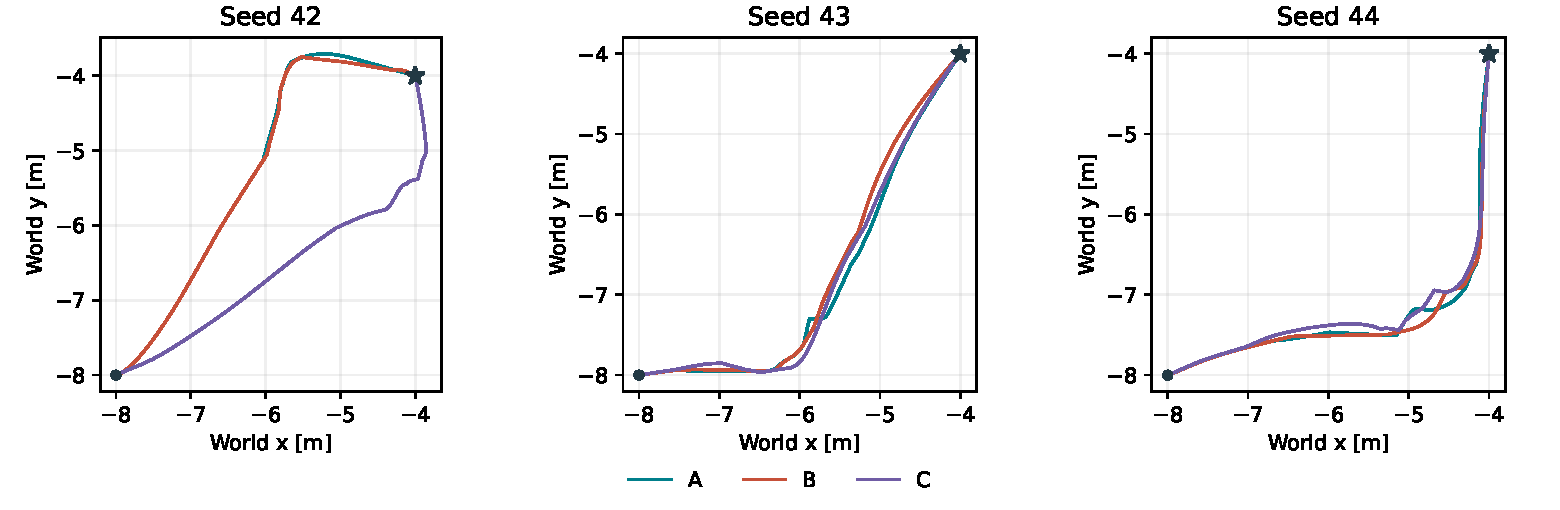
\includegraphics[width=\linewidth]{figures/ch19_navigation.pdf}
\caption{三个随机世界中的圆心轨迹，统一画在 world 坐标中，圆点为起点、星号为目标。
三种路线使用同一世界和目标，障碍净空由完整几何计算。}
\end{minipage}\end{center}
\section{分别计算定位误差、短时漂移与跟踪误差}
\subsection{先把估计位姿放进同一个世界坐标系}
用第 02 章的位姿变换记号 $T=(R,p)$，其作用是 $q\mapsto Rq+p$。
记真实位姿为 $T_i^w$，估计 odom 位姿为 $O_i$，该时刻最近可用的 map/odom 对齐为 $M_i$，
则地图中的估计位姿为 $\widehat T_i=M_iO_i$。
地图原点可以任意选择，先用第一帧确定一个固定对齐
\[
 G=T_0^w(\widehat T_0)^{-1},\qquad \widetilde T_i=G\widehat T_i.
\]
代入 $i=0$ 可见 $\widetilde T_0=T_0^w$，之后对齐 $G$ 保持不变。
这样消除的是初始坐标选择，后续累积的定位误差仍会反映在比较中。

\textbf{绝对轨迹误差}（ATE）在本章取平移部分：
\[
 e_i^{\rm ATE}=\operatorname{pos}(\widetilde T_i)-\operatorname{pos}(T_i^w),\qquad
 \mathrm{ATE}_{\rm RMS}=\sqrt{\frac1N\sum_i\|e_i^{\rm ATE}\|^2}.
\]
\code{pos} 表示取位姿中的位置向量。平方消去误差方向的正负，平均反映整段轨迹，开方后单位恢复为米。
例如两个位置误差为 $(0.01,0)$ 和 $(0,0.02)$ m，RMS 为 $\sqrt{(0.01^2+0.02^2)/2}\approx0.01581$ m。

\subsection{用相对运动检查一秒内积累的误差}
\textbf{相对位姿误差}（RPE）先比较两帧之间的运动。
真实与估计的相对变换分别为
\[
 D_{ij}=(T_i^w)^{-1}T_j^w,\qquad\widehat D_{ij}=O_i^{-1}O_j,\qquad
 E_{ij}=D_{ij}^{-1}\widehat D_{ij}.
\]
若两种运动相同，$E_{ij}$ 为单位变换。
展开第 02 章的逆变换和复合式，真实相对平移是
$R_i^T(p_j-p_i)$，表示“从第 $i$ 帧车身看，第 $j$ 帧移动到哪里”。
估计相对平移同样计算；再求两种相对变换之间的误差。
本章选择 $t_j-t_i=1$ s，取 $\|\operatorname{pos}(E_{ij})\|$ 的 RMS。
实现使用\textbf{连续 odom 位姿}计算 RPE，用带地图校正的位姿计算 ATE，分别观察短时运动与整体定位。

例如方向均为零，真值一秒前进 1 m、估计前进 1.02 m，平移 RPE 为 0.02 m。
给所有估计位姿左乘同一个固定变换 $H$，相对运动仍是
$(HO_i)^{-1}(HO_j)=O_i^{-1}O_j$，所以 RPE 对固定坐标原点的选择不敏感。

\subsection{跟踪误差与物理净空}
跟踪误差比较相同时间戳、同一 odom 系的观测位置与控制参考：
\[
 e_i^{\rm track}=p_i^{\rm odom}-p_{r,i}^{\rm odom}.
\]
它回答控制器是否跟上了自己使用的参考。
在已经对齐的一维例子中，某时刻估计位置与参考都为 1.1 m、真实位置为 1.0 m，跟踪误差为零，而估计相对真值仍偏了 0.1 m。
因此要分别查看定位和跟踪曲线。
\code{check_ch19.py} 按精确时间戳配对样本；RPE 只使用能找到一秒后对应样本的时刻。

真实圆盘净空为 $d_{\rm true}(p)-r$，其中 $d_{\rm true}$ 是真值圆心到完整障碍边界的最短距离，
计算方法见第 03 章。它检查实际外形离障碍还有多远；规划 ESDF 则描述当前观测地图中的距离。
评价还记录到达时间、停车次数、规划与控制耗时，这些量一起描述导航过程。

\section{读懂三条路线的对照结果}
\begin{center}\small
\begin{tabular}{lrrrrr}\toprule
路线/种子 & 到达/s & ATE/mm & 跟踪/mm & 净空/m & 停车\\\midrule
A/42 & 20.80 & 0.00 & 0.00 & 0.444 & 10\\
B/42 & 24.05 & 0.00 & 0.41 & 0.406 & 6\\
C/42 & 26.44 & 5.40 & 2.02 & 0.370 & 6\\
A/43 & 26.18 & 0.00 & 0.00 & 0.481 & 13\\
B/43 & 24.02 & 0.00 & 0.46 & 0.474 & 6\\
C/43 & 24.91 & 4.95 & 2.04 & 0.417 & 6\\
A/44 & 24.52 & 0.00 & 0.00 & 0.530 & 7\\
B/44 & 27.61 & 0.00 & 0.38 & 0.574 & 7\\
C/44 & 28.23 & 5.76 & 1.76 & 0.435 & 7\\
\bottomrule\end{tabular}
\end{center}
表中 ATE 和跟踪均为 RMS，净空为全程最小真实圆盘净空。
A/B 采用真值定位，零 ATE 是该输入模式的定义；A 的理想点设定用于建立几何基线。
C 的三次一秒平移 RPE 为 2.57、2.21、2.55 mm。
B/C 的 MPC 在这组运行中均完成求解；停车主要发生在新地图使旧区域失效或局部候选未通过时。
查看停车前后的状态，可以理解参考接续与重新静止起步如何配合。

这九组在三个固定随机世界中均到达目标，碰撞尝试为零。
规划 P95 耗时为 6.96--10.13 ms，B/C 的 MPC P95 为 0.38--0.46 ms。
规划计时包括局部路线、走廊和轨迹求解；地图回调中的膨胀与 ESDF、消息传输和显示另行耗时。
换用更长路线或更密集障碍时，应重新记录这些阶段的时间分布。

初始未知格约占 88.9\%--92.9\%，到达时仍有约 74.7\%--76.4\% 未知。
机器人只需逐步看清本次任务经过的区域；完整地图覆盖率与到达目标是不同的评价目标。
脚本还保存逐时刻定位、跟踪、状态和 QP 数据。汇总数据见：
\begin{center}\code{textbook/data/ch19_navigation.csv}\end{center}
相同种子复现几何和噪声流；消息调度及墙钟预算会改变具体重规划时刻，因此应比较统计量与状态过程。

可把下一组实验改成长窄通道、激光低重叠或凹形遮挡场景，观察局部目标为何停滞；
需要回环时则设置返回起点的路线，并结合第 10 章检查地图校正。
在 RViz 中同时观察观测地图、注册点云、选定里程计、局部路径和走廊，逐层定位问题。

\section{通过一份配置选择全向或阿克曼模型}
为了集中比较模型，第 04、15--17 章的平坦映射模块还提供一个停止到停止的导航入口。
机器人先静止规划一段，在途中使用对应反馈控制，完成后再接受新目标。
\begin{lstlisting}[language=bash,numbers=none]
mkdir -p tmp
cp ros2_ws/src/motion2d_bringup/config/flat_vehicle.yaml \
  tmp/vehicle.yaml
ros2 launch motion2d_bringup flat_vehicle.launch.py \
  rviz:=true config:="$PWD/tmp/vehicle.yaml"
\end{lstlisting}
在复制出的配置中编辑顶层 \code{vehicle.model} 为 \code{inertial} 或 \code{ackermann}，
\code{vehicle.localization} 为 \code{truth} 或 \code{slam}，然后重启。
launch 将物理参数同时传给仿真和规划控制；文件中的其余节点参数遵循 ROS 参数格式。

\begin{center}\small
\begin{tabular}{lll}\toprule
内容 & 全向惯性 & 阿克曼\\\midrule
平坦输出 & $(p_x,p_y,\psi)$ & $(p_x,p_y)$，前进支路\\
规划变量 & 路点、时长 & 正切向长度、时长\\
参考物理量 & 力、力变化率 & 力、转角、转向速率、侧向加速度\\
控制输入 & $F_x,F_y,\tau$ & $F,r_\delta$\\
朝向参考 & 保持起步 yaw & 路径切向，末端匹配目标 yaw\\\bottomrule
\end{tabular}\end{center}
全向后端由 \code{planning.backend} 选择 MINCO 或 Spline，控制使用前馈 PD。
阿克曼使用第 16 章的正则几何路径与停车进度，控制使用第 17 章的小车反馈。
该入口侧重模型与动力学约束；前面的全向 MPC 和运动中参考接续仍使用 \code{ch19.launch.py}。

\subsection{为反馈留出执行器余量}
默认物理力上限 2 N，参考规划上限 1 N；物理转角/速率为 0.6 rad、1 rad/s，参考上限为 0.5 rad、0.7 rad/s。
全向参考再限制力变化率 2 N/s，阿克曼参考限制侧向加速度 0.8 m/s$^2$，两者速度上限为 0.7 m/s。
软惩罚从规划上限的 85\% 开始起作用，连续界按完整规划上限检查。
剩余执行器能力供反馈消除偏差，实际指令仍按物理上限限幅。

默认圆盘半径 0.4 m，配置栅格再留 0.15 m 跟踪余量；阿克曼圆盘中心与状态点均在后轴。
truth 模式使用扫描观测建图；slam 模式使用激光、IMU 和关键帧地图。
阿克曼反馈还读取显式转角编码器，估计器仍从激光和 IMU 获取运动信息。

\section{从观测就绪到未来起步}
恢复仿真后给一个近目标：
\begin{lstlisting}[language=bash,numbers=none]
ros2 service call /sim/pause std_srvs/srv/SetBool '{data: false}'
# Truth localization: start (-8,-8), goal (-6,-7.7), yaw=0.
ros2 topic pub --once /goal_pose geometry_msgs/msg/PoseStamped \
  '{header: {frame_id: map}, pose: {
     position: {x: -6.0, y: -7.7}, orientation: {w: 1.0}}}'
ros2 topic echo /flat/status
\end{lstlisting}
SLAM 模式以第一帧为地图原点，同一相对目标为 $(2,0.3)$ m。
当前配置取初始 yaw 为零；目标需包含平面四元数，阿克曼用它约束末端朝向，全向保持起步朝向。

初始扫描后可能看到 \code{waiting_observed_free_start}。
这是因为一次自由观测的概率 0.4 还高于规划自由阈值 0.35。
由第 07 章的 log-odds 累加，两次相同自由证据给出
\[
 L_2=2\ln\frac{0.4}{0.6},\qquad
 p_2=\frac{e^{L_2}}{1+e^{L_2}}=\frac{(2/3)^2}{1+(2/3)^2}=\frac4{13}\approx0.308.
\]
重复证据会把格子推到自由阈值以下；关键帧地图则在新增关键帧后更新这些证据。
因此应先观察扫描、地图和状态，再等待可通行起点形成。

只在速度、角速度和阿克曼转角接近零时开始求解，默认预算 1 s。
求解完成后等待一条时间戳晚于求解完成时刻的新里程计，再以它的 stamp 加 0.3 s 安排起步。
这样执行起点来自新观测，而不是计算期间排队的旧数据。
曲线和区域仍按同一 map/odom 变换冻结，新地图使区域失效时则清空参考并制动。

\begin{lstlisting}[language=bash,numbers=none]
ros2 topic pub --once /flat/stop std_msgs/msg/Empty '{}'
ros2 service call /sim/reset std_srvs/srv/Trigger '{}'
\end{lstlisting}
停车、reset 或非法目标会清空旧参考。里程计新鲜而激光、地图或转角过期时，使用新状态产生限幅制动。
里程计超过 120 ms 时改用零输入：此时旧速度已无法可靠描述当前运动，持续按旧方向施力可能使车反向加速。
恢复观测后再根据当前状态重新起步。

阿克曼曲线通过 \code{/flat/ackermann_trajectory} 发布；每段保存无量纲几何参数、物理时长和绝对起点。
空曲线表示撤销。\code{/flat/reference} 为当前参考里程计，RViz 中可同时查看参考、实际位姿、地图与凸区域。

\section{用配置实验理解模型约束}
启动对应配置后，从仓库根目录运行四组模型与定位组合：
\begin{lstlisting}[language=bash,numbers=none]
/usr/bin/python3 scripts/check_flat_vehicle.py \
  --model ackermann --localization truth --output tmp/flat_check
\end{lstlisting}
脚本执行 reset、推进和暂停。改变脚本参数的同时，要重启匹配的 launch 配置。
固定 seed42，世界 $20\times20$ m、8 圆/8 多边形；质量 1 kg、半径 0.4 m，
720 束/10 Hz 激光、每束标准差 0.01 m、200 Hz IMU。相对目标为 $(2,0.3)$ m，初终朝向为零。
\begin{center}\small
\begin{tabular}{llrr}\toprule
模型/定位 & 规划后端 & 参考时长/s & 峰值跟踪/mm\\\midrule
阿克曼/truth & 专用 & 7.327 & 0.680\\
全向/truth & Spline & 11.118 & 0.145\\
阿克曼/SLAM & 专用 & 7.325 & 4.046\\
全向/SLAM & MINCO & 11.115 & 4.931\\\bottomrule
\end{tabular}
\end{center}
峰值跟踪误差由同 stamp 的选定里程计与参考比较。
表中全向两组还使用了不同后端；若要单独研究定位影响，应固定同一个后端再重复实验。
汇总数据见：
\begin{center}\code{textbook/data/flat_vehicle_validation.csv}\end{center}

将规划转角上限改成 0.005 rad，并对同一换道目标运行带 \code{--expect-failure} 的检查。
该几何候选的转角上界会超限，执行曲线保持为空。
由 $\delta=\arctan(L\kappa)$，转角由曲率决定，单纯延长时长保持 $\kappa$ 不变；
应改变路线形状、路点朝向或可用转角。
相比之下，同一几何下减慢进度可以降低纵向惯性力和转向速率，具体比例见第 16 章。

\section{练习：沿着一条消息追踪整个闭环}
\begin{enumerate}
\item \textbf{代码 ch19-1：}补全首 p/v/a 比较。用旧曲线在 1.5 s 的解析结果，构造只改速度的候选并检查接收结果。
\item 按时间表依次查询未来、当前、交接后；解释为什么查询函数与推进函数应分开。
\item 手算本章 $90^\circ$ 旋转的曲线首点和速度，再将常数系数与高次系数分别变回 map 核对。
\item 用剩余路长和线性插值截断一条 A* 路线；更改未知区域边界，观察局部目标如何移动。
\item 推导 $p(T/2)=D/2+5v_0T/32$，比较 $D=1,v_0=0.5$ 时两个时长，说明备用方案为何仍需重新检查走廊。
\item \textbf{代码 ch19-2：}按仿真时间补全周期触发条件，检查首次、暂停、周期边界、待交接和回退。
\item 删去候选的一个区域，跟踪发送、拒绝与旧参考继续执行；再停掉扫描，观察里程计仍更新时的传感器年龄判断。
\item 用同一组样本分别算 ATE、RPE 和跟踪 RMS，解释它们的坐标、时间配对和单位。
\item \textbf{配置 ch19-3：}每次只改变质量、规划力或转角上限，记录参考时长、连续界、跟踪误差与状态。为一个超限案例提出几何或时间上的修改。
\end{enumerate}
练习编译入口与手算提示见 \code{exercises/ch19/README.md}。
